\documentclass[tikz,border=6pt]{standalone}
\usepackage[T1]{fontenc}
\usepackage{lmodern}
\usepackage{amsmath,amssymb}
\usetikzlibrary{positioning,arrows.meta,fit,calc}
% Design of koblitz-n83-closure-indexlift-20261019 (frozen protocol.json). Not a result.
\begin{document}
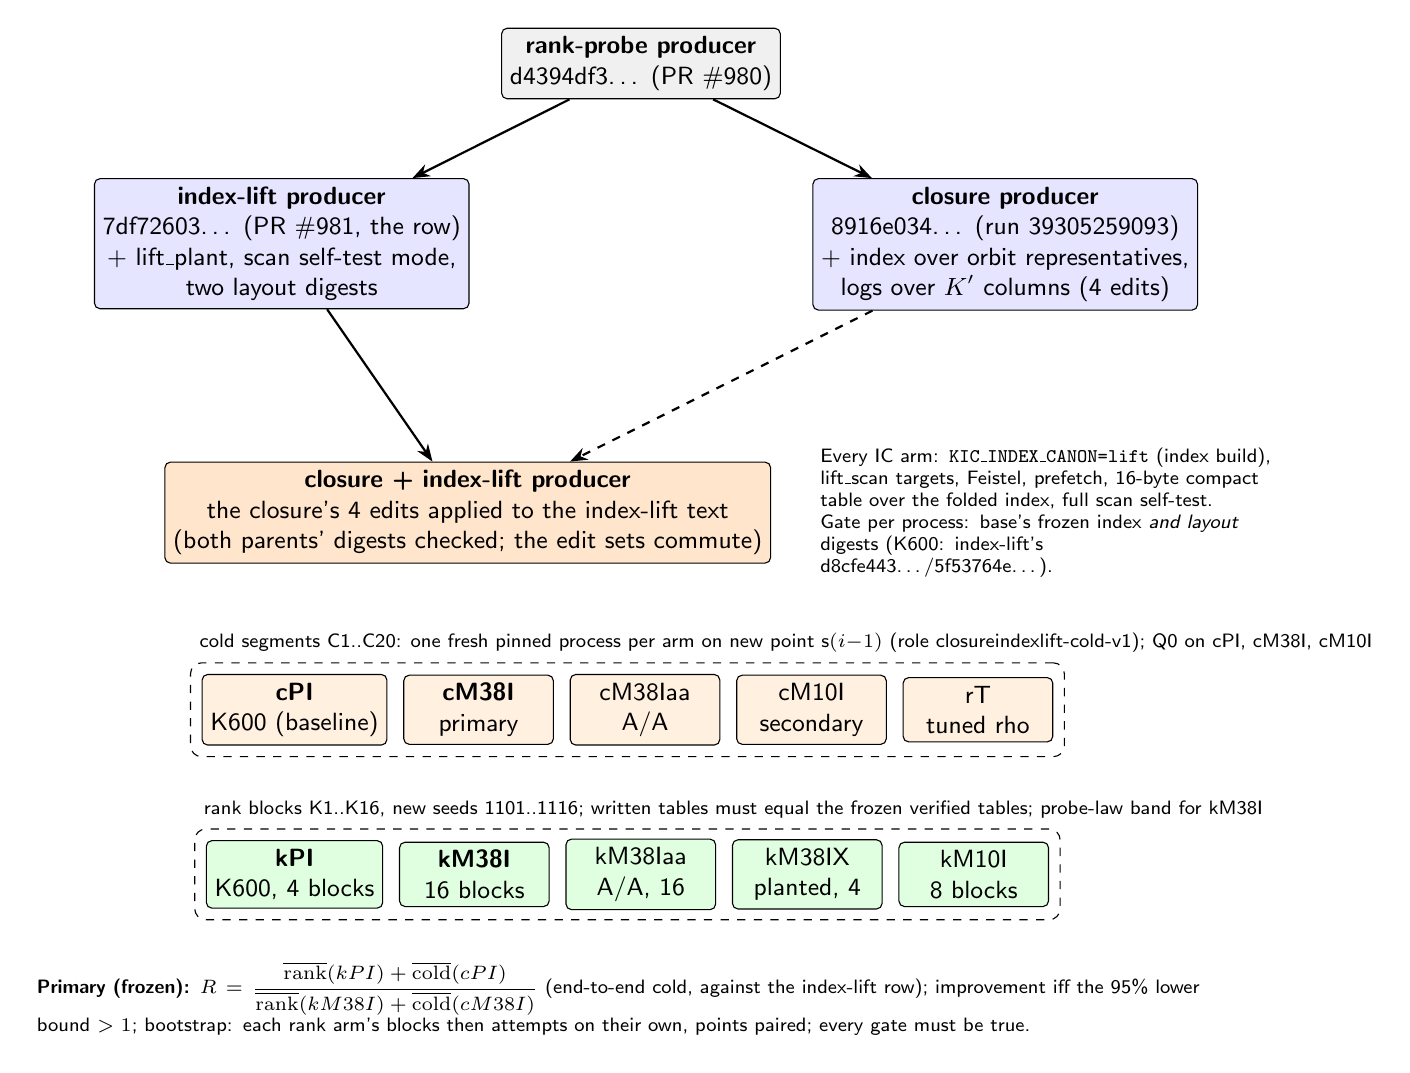
\begin{tikzpicture}[
  font=\sffamily\small,
  box/.style={draw, rounded corners=2pt, align=center, minimum height=8mm, inner sep=3pt},
  base/.style={box, fill=gray!12},
  add/.style={box, fill=blue!10},
  arm/.style={box, fill=orange!12, minimum width=19mm},
  rank/.style={box, fill=green!12, minimum width=19mm},
  arr/.style={-{Stealth[length=2.2mm]}, thick},
  note/.style={align=left, font=\sffamily\scriptsize}
]
\node[base] (rp) {\textbf{rank-probe producer}\\d4394df3\ldots\ (PR \#980)};
\node[add, below left=10mm and 4mm of rp] (il) {\textbf{index-lift producer}\\7df72603\ldots\ (PR \#981, the row)\\+ lift\_plant, scan self-test mode,\\ two layout digests};
\node[add, below right=10mm and 4mm of rp] (cl) {\textbf{closure producer}\\8916e034\ldots\ (run 39305259093)\\+ index over orbit representatives,\\ logs over $K'$ columns (4 edits)};
\node[box, fill=orange!20, below=46mm of rp, xshift=-22mm] (ci) {\textbf{closure + index-lift producer}\\the closure's 4 edits applied to the index-lift text\\(both parents' digests checked; the edit sets commute)};
\draw[arr] (rp) -- (il); \draw[arr] (rp) -- (cl); \draw[arr] (il) -- (ci); \draw[arr, dashed] (cl) -- (ci);
\node[note, right=5mm of ci, text width=58mm] {Every IC arm: \texttt{KIC\_INDEX\_CANON=lift} (index build),\\lift\_scan targets, Feistel, prefetch, 16-byte compact\\table over the folded index, full scan self-test.\\Gate per process: base's frozen index \emph{and layout}\\digests (K600: index-lift's d8cfe443\ldots/5f53764e\ldots).};
\node[arm, below=14mm of ci, xshift=-22mm] (cP) {\textbf{cPI}\\K600 (baseline)};
\node[arm, right=2mm of cP] (cM) {\textbf{cM38I}\\primary};
\node[arm, right=2mm of cM] (cMa) {cM38Iaa\\A/A};
\node[arm, right=2mm of cMa] (cT) {cM10I\\secondary};
\node[arm, right=2mm of cT] (rT) {rT\\tuned rho};
\node[draw, dashed, rounded corners, fit=(cP) (rT), inner sep=4pt, label={[note, anchor=south west]north west:{cold segments C1..C20: one fresh pinned process per arm on new point s$(i{-}1)$ (role closureindexlift-cold-v1); Q0 on cPI, cM38I, cM10I}}] (cold) {};
\node[rank, below=12mm of cP] (kP) {\textbf{kPI}\\K600, 4 blocks};
\node[rank, right=2mm of kP] (kM) {\textbf{kM38I}\\16 blocks};
\node[rank, right=2mm of kM] (kMa) {kM38Iaa\\A/A, 16};
\node[rank, right=2mm of kMa] (kMX) {kM38IX\\planted, 4};
\node[rank, right=2mm of kMX] (kT) {kM10I\\8 blocks};
\node[draw, dashed, rounded corners, fit=(kP) (kT), inner sep=4pt, label={[note, anchor=south west]north west:{rank blocks K1..K16, new seeds 1101..1116; written tables must equal the frozen verified tables; probe-law band for kM38I}}] (rkb) {};
\node[note, below=4mm of rkb, text width=150mm] {\textbf{Primary (frozen):}
$R=\dfrac{\overline{\mathrm{rank}}(kPI)+\overline{\mathrm{cold}}(cPI)}{\overline{\mathrm{rank}}(kM38I)+\overline{\mathrm{cold}}(cM38I)}$ (end-to-end cold, against the index-lift row);
improvement iff the 95\% lower bound $>1$; bootstrap: each rank arm's blocks then attempts on their own, points paired; every gate must be true.};
\end{tikzpicture}
\end{document}
